\documentclass[margin=5mm]{standalone}
\usepackage[utf8]{inputenc}
\usepackage{tikz}

\usetikzlibrary{calc, positioning}
\usetikzlibrary{arrows.meta}
\usetikzlibrary{matrix}
\usetikzlibrary{shadows}
\usepgflibrary{shapes.misc}
\usepgflibrary{{shapes.geometric}}

\pgfdeclarelayer{shadow} 
\pgfsetlayers{shadow,main}
\def\shadowradius{3pt}


\def\mw{1.5cm}
\def\mh{1cm}
\def\trianglecoordinate{2mm}

\tikzstyle{component} = [draw, fill=white, minimum width=\mw, minimum height=\mh, align=center]

\tikzset{
    border/.style = { 
        draw, rectangle, minimum width=\mw, minimum height=\mh, ultra thick, align=center
    },
    Component/.pic = {
        \node [border](-edge){#1}; 
        \draw[thick] ([xshift=\trianglecoordinate] -edge.south) -- ([yshift=\trianglecoordinate] -edge.south);
        \draw[thick] ([xshift=-\trianglecoordinate] -edge.south) -- ([yshift=\trianglecoordinate] -edge.south);
        \draw[thick] (-edge.south) |- ++(-3mm, -4mm) node[xshift=-2mm, yshift=-1mm] {T}; 
    },
}

\tikzset{
    clockborder/.style = { 
        trapezium, trapezium angle=60, minimum width=1cm, draw, ultra thick
    },
    Clock/.pic = {
        \node [clockborder, shape border rotate=-180](-clockedge){#1};
        \draw[very thick] (-clockedge.east) -- ++(2cm, 0cm);
        \def\sft{0.5}
        \foreach \x in {0, 0.5, 1, 1.5}{
            \draw[very thick] (\x + \sft, 0.1) -| ++(0.25cm, 0.25cm) -| ++ (0.25cm, -0.25cm);
        }
    },
}

\begin{document}
    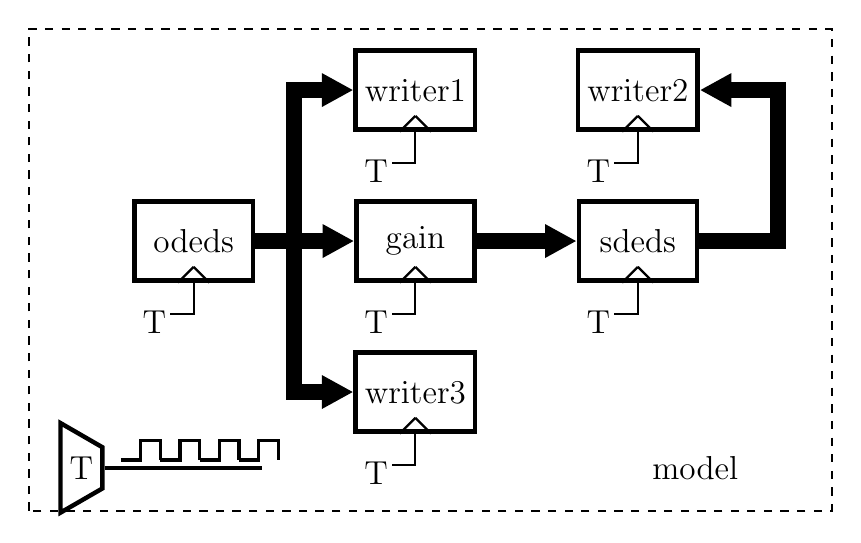
\begin{tikzpicture}[every node/.style={font=\large}]
        % Place the blocks 
        \matrix (m) [matrix of nodes, ampersand replacement=\&, column sep = 1.25cm, row sep = 0.1cm, nodes={anchor=center}]{
                                            \& \draw pic (b1) {Component={writer1}}; \& \draw pic (b2) {Component={writer2}}; \\
        \draw pic (b3) {Component={odeds}};    \& \draw pic (b4) {Component={gain}}; \& \draw pic (b5) {Component={sdeds}}; \\
                                            \& \draw pic (b6) {Component={writer3}}; \&                                  \\
        };
        % Draw connections 
        \begin{scope}[line width=2mm, >={Triangle[width=4mm,length=4mm]}]
            \def\shiftamount{0.5mm};
            \draw[-] (b3-edge.east) -- ++(0.5cm, 0cm) coordinate(a);
            \draw[->] (a) |- (b1-edge.west);
            \draw[->] (a) |- (b4-edge.west);
            \draw[->] (a) |- (b6-edge.west);
            \draw[->] (b4-edge.east) -- (b5-edge.west);
            \draw[-] (b5-edge.east) -- ++(1cm, 0cm) coordinate(b);
            \draw[->] ([yshift=-1mm] b) |- (b2-edge.east);
        \end{scope}

        % \Place clock 
        \begin{scope}[shift={(-4.25cm, -2.5cm)}]
            \draw pic(clk) {Clock={T}} ;
        \end{scope}

        %  Draw rectangle 
        \draw[dashed, thick] ([xshift=-0.25*\mw, yshift=-0.25*\mh] clk-clockedge.south west) rectangle ([xshift=3*\mw, yshift=0.25*\mh] b1-edge.north east);
        \draw (clk-clockedge.east) node[yshift=0*\mh, xshift=5*\mw]{model};
    \end{tikzpicture}
\end{document}